\documentclass[11pt]{article}
\usepackage[margin=1in]{geometry}
\usepackage{booktabs}
\usepackage{graphicx}
\usepackage{microtype}

\title{Fine-mapped eQTL evaluation using XQTL mega-eQTL data}
\author{}
\date{}

\begin{document}
\maketitle

\section{Overview}
This analysis applies the variant-effect benchmark in \texttt{eqtl.tex} to
six cell-type mega-eQTL fine-mapping datasets supplied as Sum of Single
Effects (SuSiE) posterior
inclusion probabilities (PIPs) for expression quantitative trait loci
(eQTLs). In this report, XQTL names this six-group source. The groups are astrocytes (Ast),
excitatory neurons (Exc), inhibitory neurons (Inh), microglia (Mic),
oligodendrocyte precursor cells (OPC), and oligodendrocytes (Oli). The input
does not contain an endothelial group. We compare these results with the
existing singlebrain fine-mapping, using its broad Ast, Ext, IN, MG, OPC, and
OD panels, respectively.

\section{Methods}
For both data sources, gene identifiers are version-normalized and matched to
the same GENCODE hg38 gene annotation. Variants are restricted to single-base
ACGT substitutions on the gene chromosome within $512\,\mathrm{kb}$ of the
gene transcription start site (TSS). Variants with PIP $>0.75$ are positives;
those with PIP $<0.01$ are negatives. The benchmark samples up to 1,000
variants from each class in each group with a fixed seed. Each model receives
a $1\,\mathrm{Mb}$ sequence window centered at the gene TSS.

The trained comparisons reuse the head-only, LoRA, and LoRA+LoCon checkpoints
and RNA track mappings in \texttt{eqtl.tex}. Native AlphaGenome mutation
effects use all available RNA-seq and CAGE tracks, followed by the same
biologically constrained track selection used in that report. Performance
includes area under the receiver operating characteristic curve (AUROC) and
average precision (AP), overall and by distance to the TSS; random AP equals
the positive prevalence within each distance bin. CAGE means Cap Analysis of
Gene Expression.

Fine-mapping agreement is computed on gene-variant keys consisting of gene,
chromosome, one-based position, reference allele, and alternate allele. Exact
high-confidence overlap uses all eligible variants and reports intersection,
Jaccard similarity, and directional recall at PIP $>0.75$. Continuous PIP
agreement is assessed on a seeded sample of up to 25,000 eligible rows per
group, matched by the same gene-variant key; Pearson and Spearman correlations
are reported for shared sampled rows. The PIP sample is used for correlation
and visualization only, not for the exact high-PIP overlap.

\section{Fine-mapping agreement}
The full scan covered 70.9--218.7 million input rows per group. After
matching to an annotated gene, requiring a single-base substitution on the
gene chromosome, and applying the TSS window, 14.3--41.2 million records per
group remained. Table~\ref{tab:xqtl_counts} gives counts and PIP classes.

\begin{table}[ht]
\centering
\scriptsize
\caption{XQTL source counts. Eligible rows satisfy the common gene, allele,
chromosome, and TSS-window filters.}
\label{tab:xqtl_counts}
\begin{tabular}{@{}lrrrr@{}}
\toprule
Group & Input rows & Eligible rows & PIP $>0.75$ & PIP $<0.01$ \\
\midrule
Astrocyte & 167,399,779 & 31,850,543 & 581 & 31,769,295 \\
Excitatory & 218,708,555 & 41,150,681 & 1,784 & 40,976,915 \\
Inhibitory & 207,868,448 & 39,394,880 & 813 & 39,281,800 \\
Microglia & 70,865,864 & 14,332,701 & 168 & 14,305,646 \\
OPC & 122,683,778 & 24,317,596 & 358 & 24,269,005 \\
Oligodendrocyte & 178,552,659 & 33,830,282 & 852 & 33,738,029 \\
\bottomrule
\end{tabular}
\end{table}

At the high-confidence threshold, exact gene-variant Jaccard similarity is
0.080--0.118 (Table~\ref{tab:overlap}). XQTL positive recall against
singlebrain is 0.28--0.37, while singlebrain positive recall against XQTL is
0.09--0.16. Thus the sources share some high-confidence calls but the two
sets are not interchangeable. On up to 25,000 randomly sampled eligible
XQTL records per group, 9,238--12,359 have an exact gene-variant match in
singlebrain. Their Spearman PIP correlations are 0.16--0.20, indicating weak
rank agreement. Pearson correlations are higher in some groups because of
the strongly zero-inflated PIP distribution and should not be interpreted as
uniform agreement across the PIP range.

\begin{table}[ht]
\centering
\scriptsize
\caption{Exact high-PIP overlap and sampled continuous-PIP agreement. Recall
columns use the named source as denominator.}
\label{tab:overlap}
\begin{tabular}{@{}lrrrrrrr@{}}
\toprule
Group & XQTL $n$ & Singlebrain $n$ & Shared & Jaccard & XQTL recall & SB recall & Spearman $r$ \\
\midrule
Astrocyte & 581 & 1,231 & 172 & 0.105 & 0.296 & 0.140 & 0.177 \\
Excitatory & 1,784 & 3,420 & 504 & 0.107 & 0.283 & 0.147 & 0.194 \\
Inhibitory & 813 & 1,838 & 236 & 0.098 & 0.290 & 0.128 & 0.187 \\
Microglia & 168 & 668 & 62 & 0.080 & 0.369 & 0.093 & 0.196 \\
OPC & 358 & 929 & 122 & 0.105 & 0.341 & 0.131 & 0.158 \\
Oligodendrocyte & 852 & 1,820 & 283 & 0.118 & 0.332 & 0.155 & 0.172 \\
\bottomrule
\end{tabular}
\end{table}

\IfFileExists{figures/eqtl_xqtl_finemap_high_pip_overlap.pdf}{
\begin{figure}[ht]
\centering
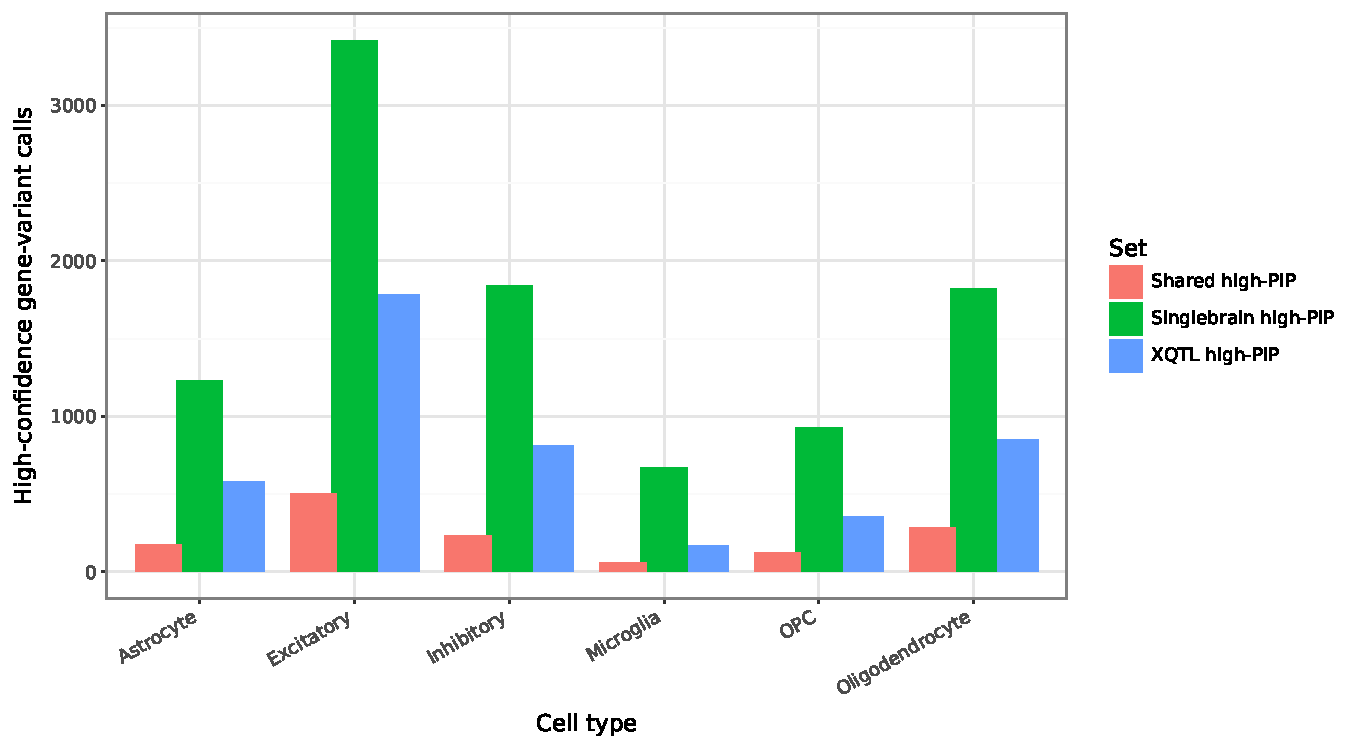
\includegraphics[width=0.95\linewidth]{figures/eqtl_xqtl_finemap_high_pip_overlap.pdf}
\caption{Counts of eligible high-PIP gene-variant calls in each source and
their exact intersection.}
\end{figure}
}{The exact overlap scan completed, but the figure is missing.}

\IfFileExists{figures/eqtl_xqtl_finemap_pip_agreement.pdf}{
\begin{figure}[ht]
\centering
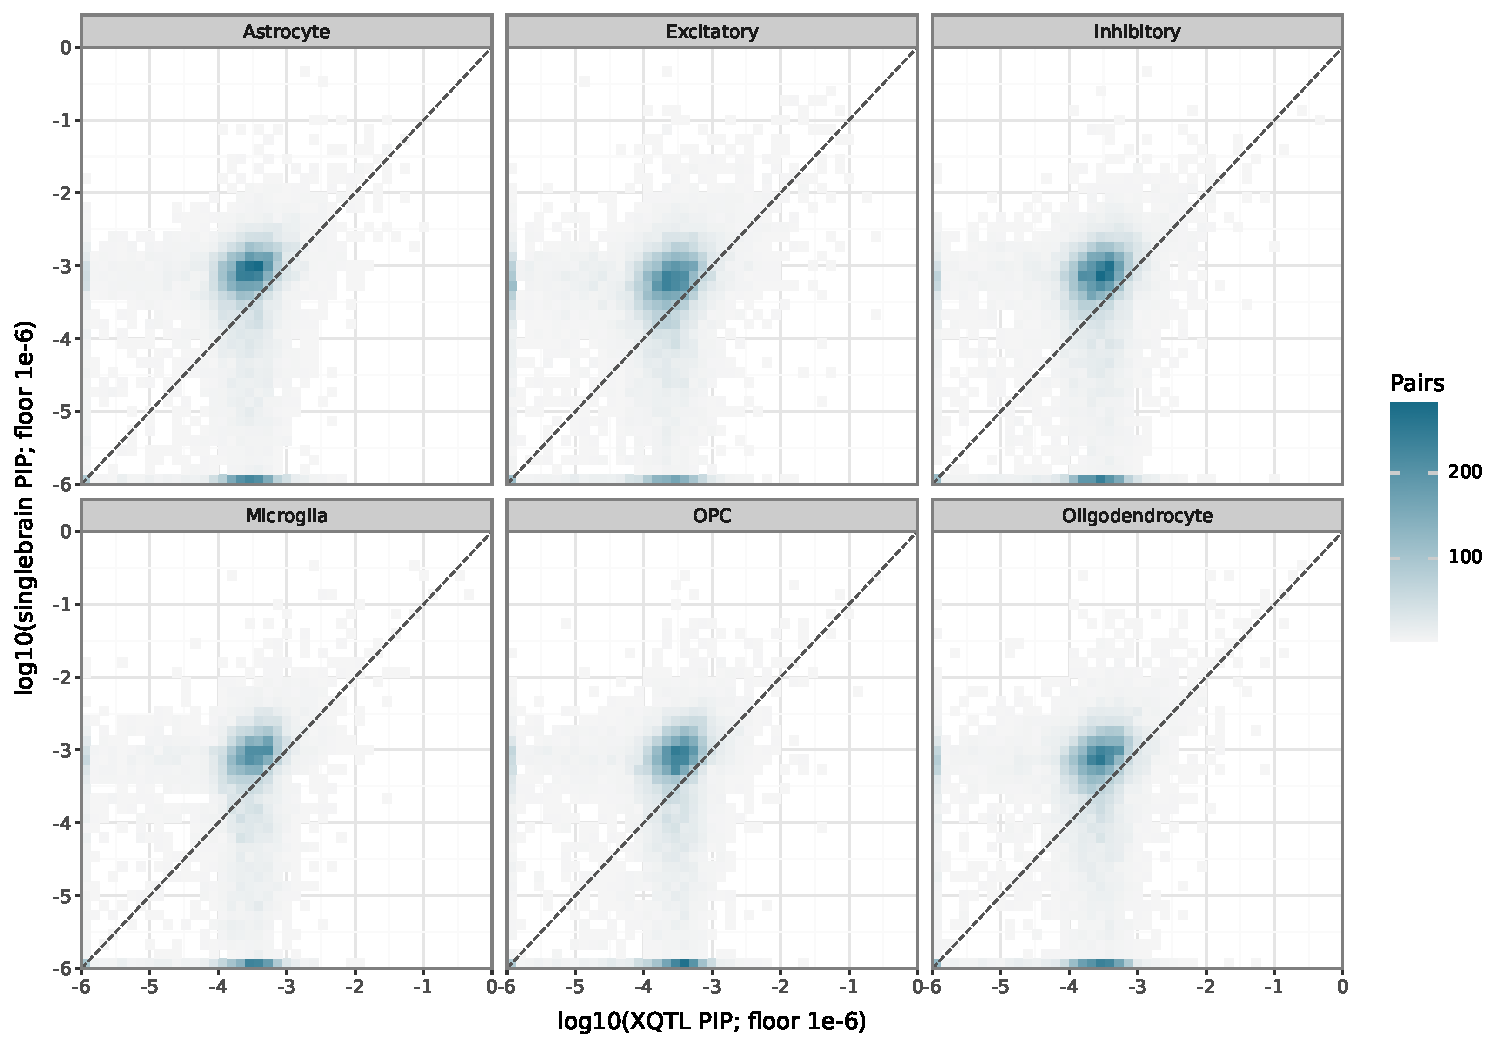
\includegraphics[width=0.95\linewidth]{figures/eqtl_xqtl_finemap_pip_agreement.pdf}
\caption{Continuous PIP agreement for sampled gene-variant pairs present in
both sources. Axes show $\log_{10}(\max(\mathrm{PIP},10^{-6}))$; the dashed
diagonal indicates equality.}
\end{figure}
}{The matched PIP sample was collected, but the figure is missing.}

\section{Variant-effect performance}
\IfFileExists{figures/eqtl_xqtl_auroc_by_distance.pdf}{
\begin{figure}[ht]
\centering
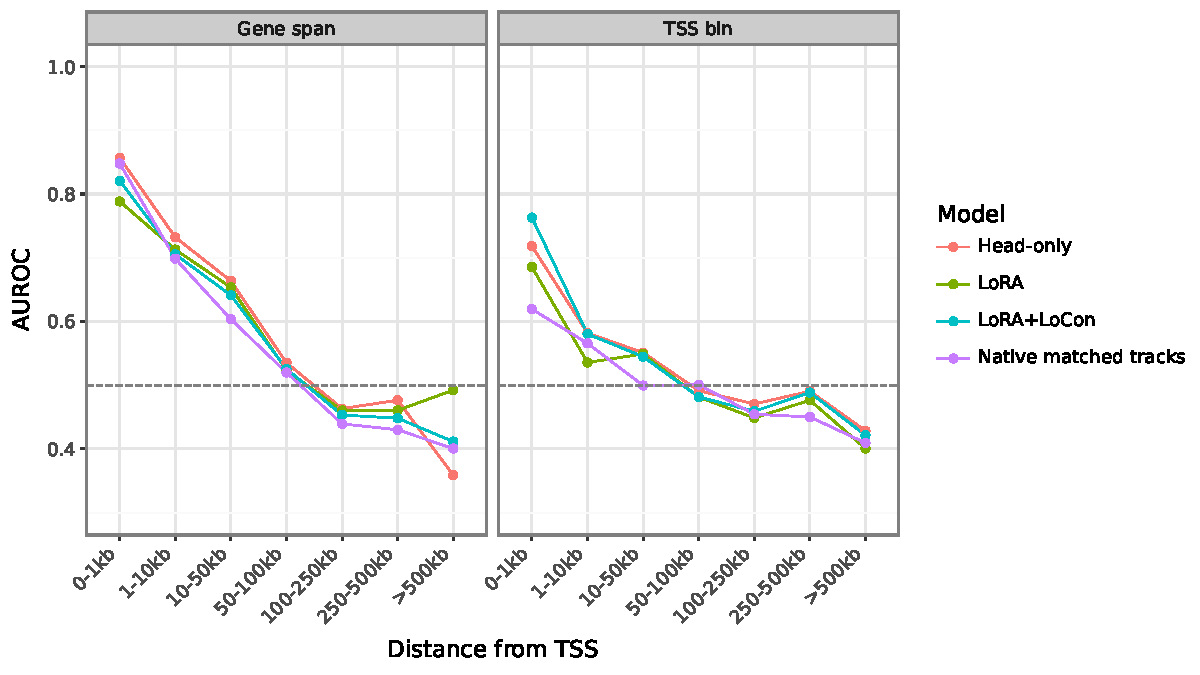
\includegraphics[width=0.95\linewidth]{figures/eqtl_xqtl_auroc_by_distance.pdf}
\caption{AUROC by absolute distance from the TSS.}
\end{figure}
}{The model and native-track runs are pending; performance results will be
inserted when scoring is complete.}

\IfFileExists{figures/eqtl_xqtl_aupr_by_distance.pdf}{
\begin{figure}[ht]
\centering
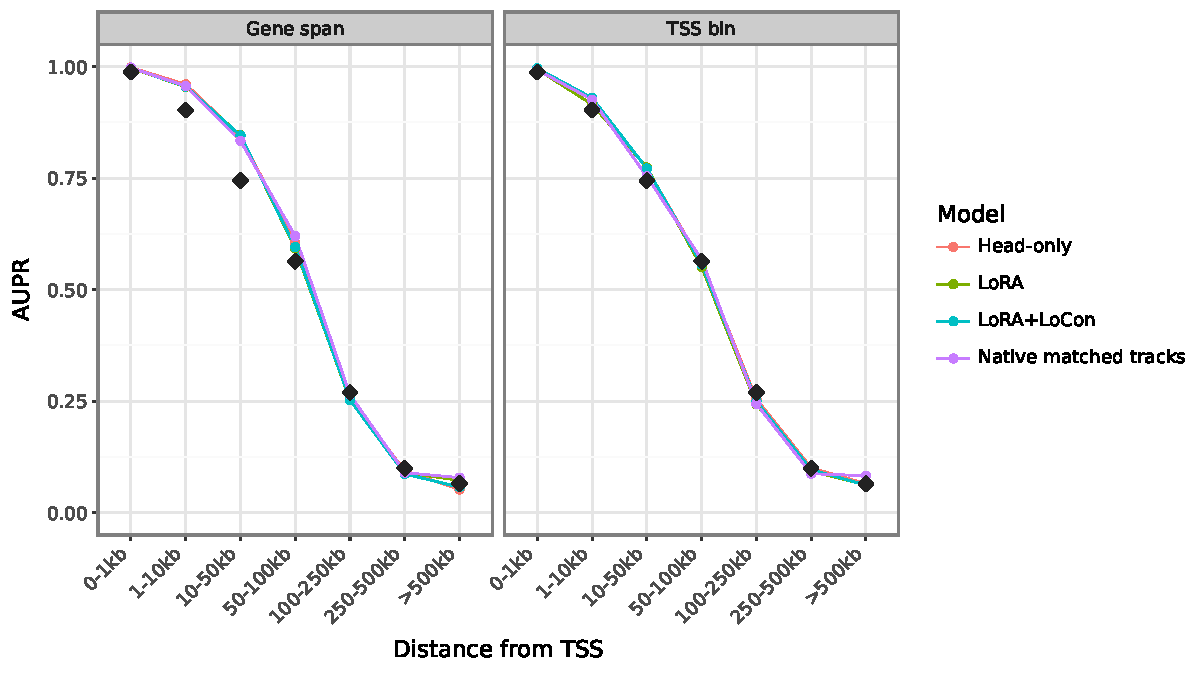
\includegraphics[width=0.95\linewidth]{figures/eqtl_xqtl_aupr_by_distance.pdf}
\caption{Average precision by absolute distance from the TSS. The random
reference is the positive prevalence in each bin.}
\end{figure}
}{ }

\end{document}
